%  !TEX root = _main.tex
\section{VOICEPEAKによる発話イントネーションの取得}\label{sec:huroku1}



\red{割合を求めるために，語句のイントネーションを求める(?????)．}

VOICEPEAKで“あなたにあいたくて”“ひかりのほう”の合成音声のプロジェクトファイルを作成した．それをテキストエディタのVisual Studio Codeで開き，成形すると，終端にNull文字のあるJSONファイルとなる．

実際に成形した後のコードの一部が\figref{json_seikei}である．この図は「あなたにあいたくて」と言わせたときのJSONファイル「な」の部分で，各項目で合成音声の声音を制御している．

イントネーションに関わる部分は，\figref{json_seikei}の“i”である．\figref{hikui}はVOICEPEAK上でイントネーションの値を最も低くしたもの，\figref{takai}はVOICEPEAK上でイントネーションの値を最も高くしたものである．\figref{hikui}の“i”を見てみると，“-1.55575704574585”，\figref{takai}の“i”を見てみると，“4.44424295425415”となっており，絶対値同士を足すと6となる．他の値についても同様であり，VOICEPEAKにおけるイントネーションの設定は，幅6の間で設定されているとわかる．


\begin{figure}[t]
    \begin{minipage}[t]{0.49\columnwidth}
        \begin{center}
            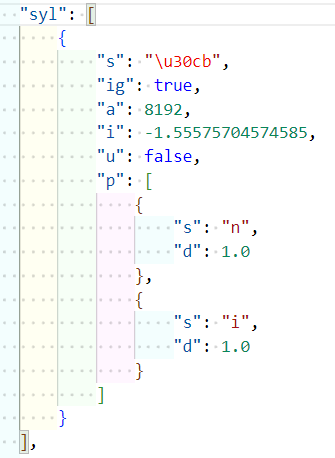
\includegraphics[width=\columnwidth]{fig/intone_hidari.png} % 図の大きさに合わせてscaleやwidth=\linewidthで調整
            \subcaption{全てのイントネーションを\\低くしたもの}
            \label{hikui}
        \end{center}
    \end{minipage}
    \begin{minipage}[t]{0.49\columnwidth}
        \begin{center}
            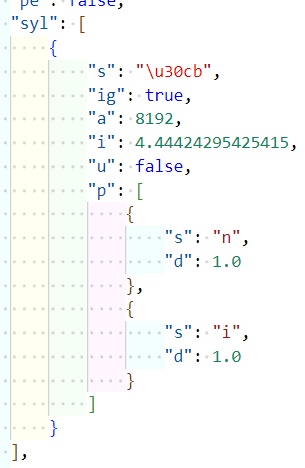
\includegraphics[width=\columnwidth]{fig/intone_migi.png}
            \subcaption{全てのイントネーションを\\高くしたもの}
            \label{takai}
        \end{center}
    \end{minipage}

    \caption{VOICEPEAKのプロジェクトファイルの中身}
    \label{json_seikei}
\end{figure}

\red{付録に回したので，もう少し加筆できる}